\chapter{Concept for an Exergame for Elderly}


\section{A Video Game Series}
\begin{figure} [ht!]
\centering
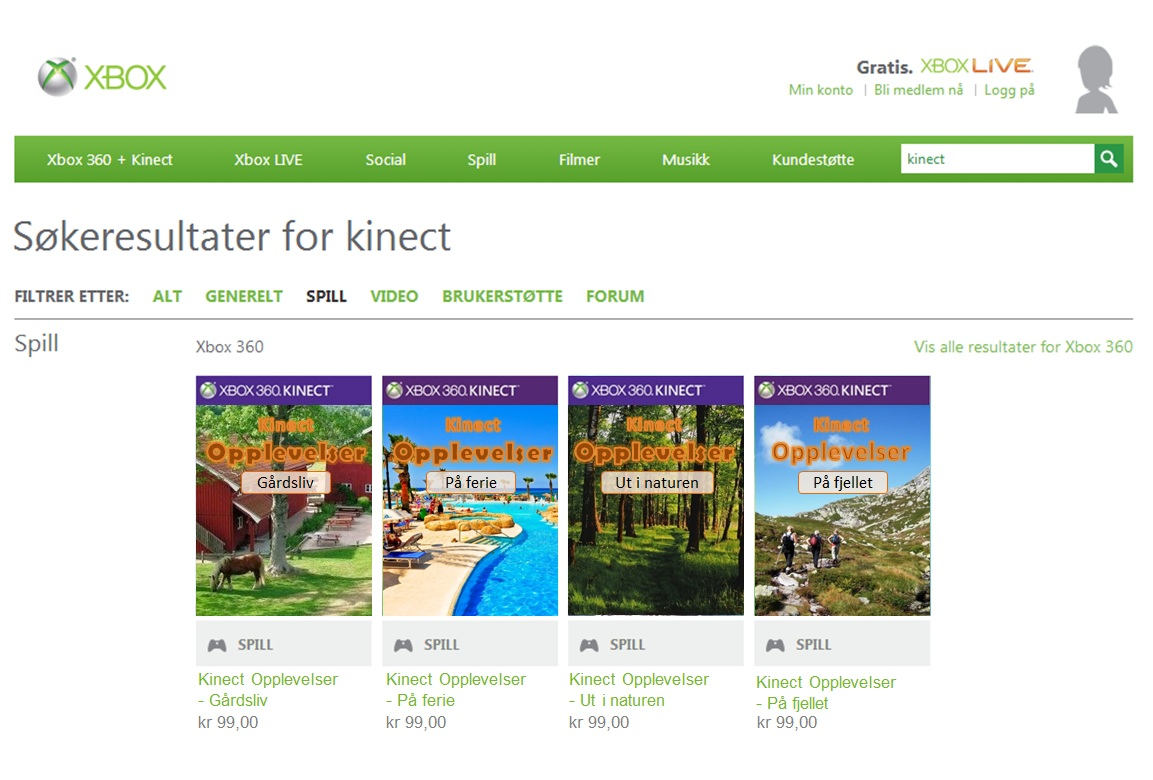
\includegraphics[scale=0.5, angle=90]{SpillXboxNYNY.jpg}
\caption[Presentation of our video game series]{A presentation of how our video game series would look like on Xbox's website [modified from \cite{XboxNettside}].}
\label{fig:videogameseries}
\end{figure}

\begin{figure} [ht!]
\centering
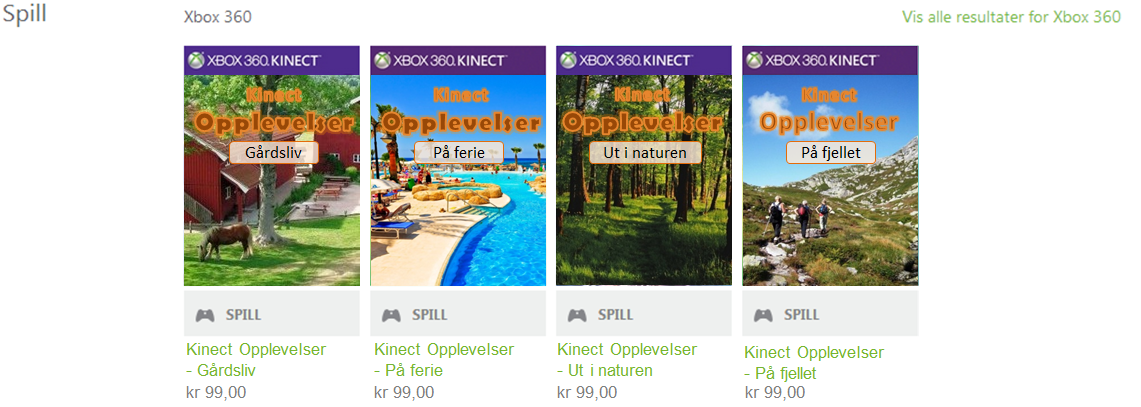
\includegraphics[scale=0.6]{SpillXboxNY.png}
\caption[Presentation of our video game series]{A presentation of how our video game series would look like on Xbox's website [modified from \cite{XboxNettside}].}
\label{fig:videogameseries}
\end{figure}

\section{Out in the Nature}

\begin{figure} [ht!]
\centering
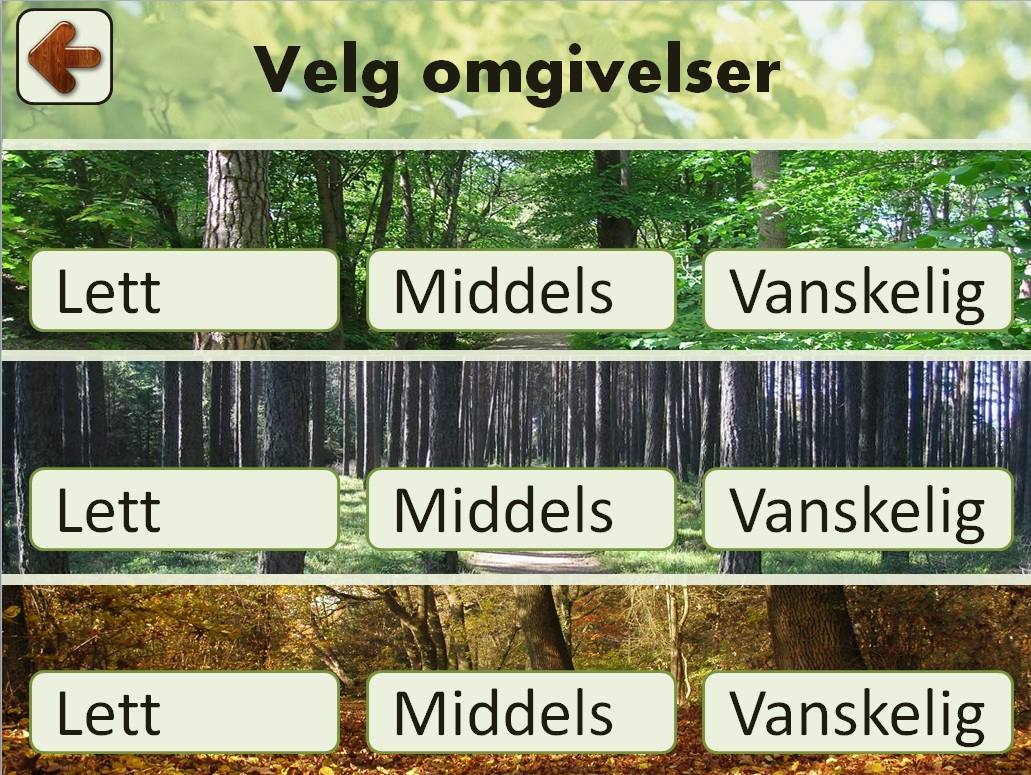
\includegraphics[scale=0.45]{VelgOmgivelser.jpg}
\caption[Choice of surroundings and difficulty]{When "Take a walk in the nature" is chosen, players will get the possibility to choose surroundings and difficulty level.}
\label{fig:omgivelseNivaa}
\end{figure}

\begin{figure} [ht!]
\centering
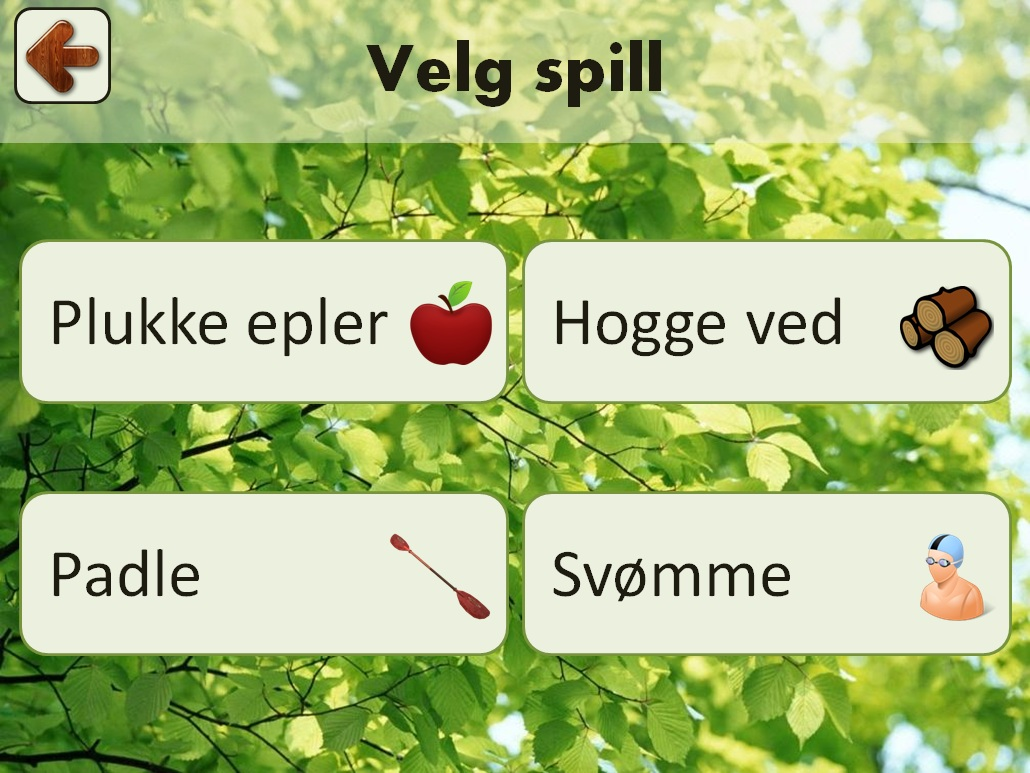
\includegraphics[scale=0.4]{VelgSpill.jpg}
\caption[The four single games]{Besides the walk in the nature the players can choose between four single games, picking apples, chopping wood, paddling, and swimming.}
\label{fig:velgSpill}
\end{figure}


\section{The Menu}

In this section we will present a proposal for a menu. The reason for doing this is based on observed problems in workshop 1 related to menus in existing video games, and also our own experience from playing. 
The general perception of the menus was that they were complex, difficult to follow, demanding to navigate through, and that they were too sensitive. 

The menu presented is a prototype developed with Microsoft PowerPoint. We had planned to develop an simple menu interface with the Kinect for Windows SDK, that we would present on workshop 2 with the Kinect sensor. However, to do this we had to buy the Kinect sensor for Windows, which costs 1 790 NOK \cite{kinectpc}. We felt that was too expensive for its purpose in this master thesis, and we therefore chose to make the inexpensive PowerPoint prototype.   

The design of our menu proposal is based upon feedback from workshop 1, and theory about designing interfaces for elderly. Simple design, distinct elements, and easy to read information is emphasised to make it user-friendly for elderly that might suffer from declined vision. It has been a focus not to have too much information in each menu step. We have therefore chosen to make a menu consisting of more steps, rather than fill few menu steps with lots of information and choices.   

We can take a look at Figure \ref{fig:velgSpill} to observe the different menu elements. We have used a different range of green colors, and a picture of green leaves as background, to create a theme related to forest and nature. The title on each step is written in a bold, black, easy to read font, on a semi-transparent light-colored background. The title is stating what choice to be made at the current step. From Section \ref{sec:designguide} we know that it is important to have an interface with visible information. Up in the left corner there is a back button, which will make it possible for users to always regret their actions.      
Farger.
Lys bakgrunn, mørk tekst.
Blad som bakgrunn.
Kontraster i forhold til omgivelsene. 

\begin{figure} [ht!]
\centering
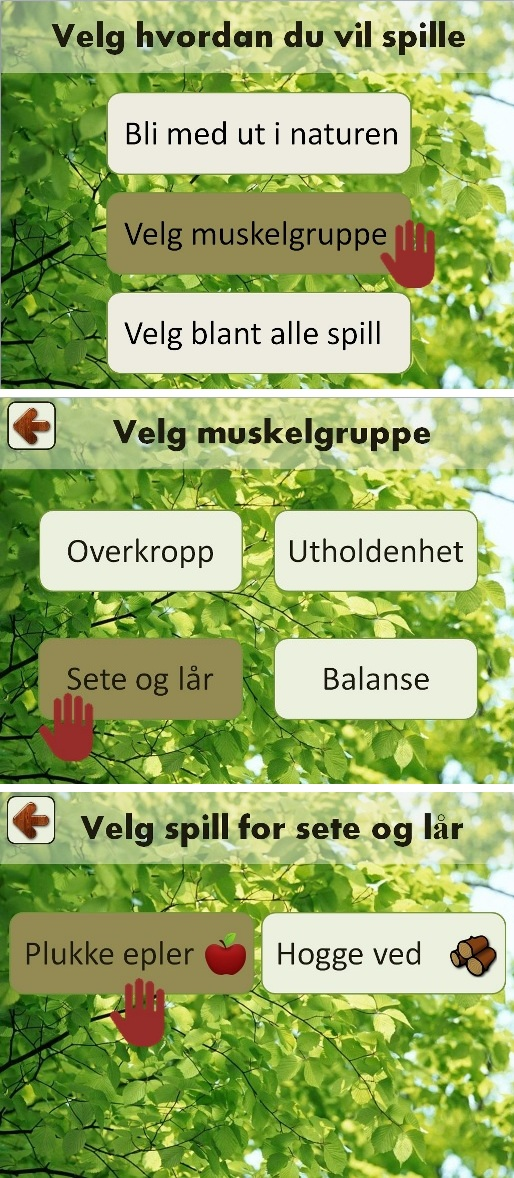
\includegraphics[scale=0.5]{menuStep1.jpg}
\caption[The menu, part one]{This figure shows the menu step by step, from the beginning to playing a single game, here picking apples. The selection of single games is a result of the chosen muscle group.}
\label{menu1}
\end{figure}

\begin{figure} [ht!]
\centering
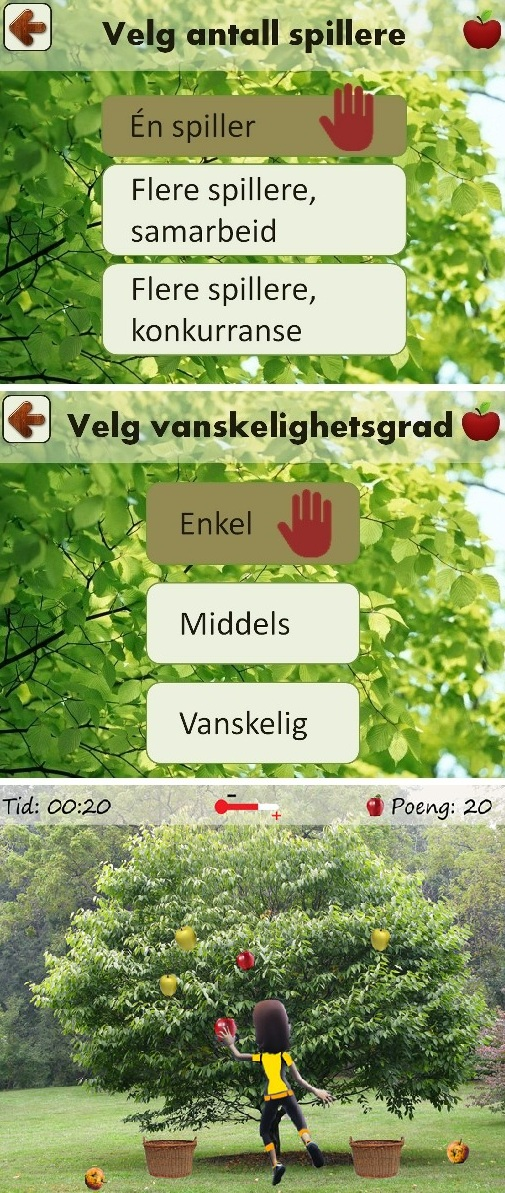
\includegraphics[scale=0.5]{menuStep2.jpg}
\caption[The menu, part two]{This figure shows the menu step by step, from the beginning to playing a single game, here picking apples. Single player game and difficulty level easy are chosen.}
\label{menu2}
\end{figure}